\section{Auswertung}
\label{sec:Auswertung}

% Durchmesser kl. Kugel: 1.5570+/-0.0010 (in cm)
% Durchmesser gr. Kugel: 1.5760+/-0.0010 (in cm)
% Volumen der kl. Kugel: 1.976+/-0.004 (in cm^3)
% Volumen der gr. Kugel: 2.050+/-0.004 (in cm^3)
% Dichte der kl. Kugel: 2.253+/-0.004 (in g/cm^3)
% Dichte der gr. Kugel: 2.416+/-0.005 (in g/cm^3)
% Gemittelte Fallzeit (hoch) kl: 12.20+/-0.13, gr: 34.75+/-0.16
% Gemittelte Fallzeit (runter) kl: 12.14+/-0.11, gr: 34.73+/-0.09
% Viskosität hoch: 1.170+/-0.013 (in mPa*s)
% Viskosität runter: 1.164+/-0.011 (in mPa*s)
% Apparaturkonstante K_gr_h: 0.02374+/-0.00030 (in mPa*cm^3/g)
% Apparaturkonstante K_gr_r: 0.02364+/-0.00025 (in mPa*cm^3/g)
% Reynoldsche Zahl Re_kl_h: 110.2+/-2.4
% Reynoldsche Zahl Re_kl_r: 111.3+/-2.0
% Reynoldsche Zahl Re_gr_h: 19.35+/-0.24
% Reynoldsche Zahl Re_gr_r: 19.46+/-0.19

% K_kl = 0.07640 (in m*Pa*cm^3/g) (gegeben)
% dichte_wasser = 0.998207 (in g/cm^3) (Internet)
% aus Plot:
% B = 1680.3669999374256
% A = 0.0038202859833589985
\begin{figure}
  \centering
  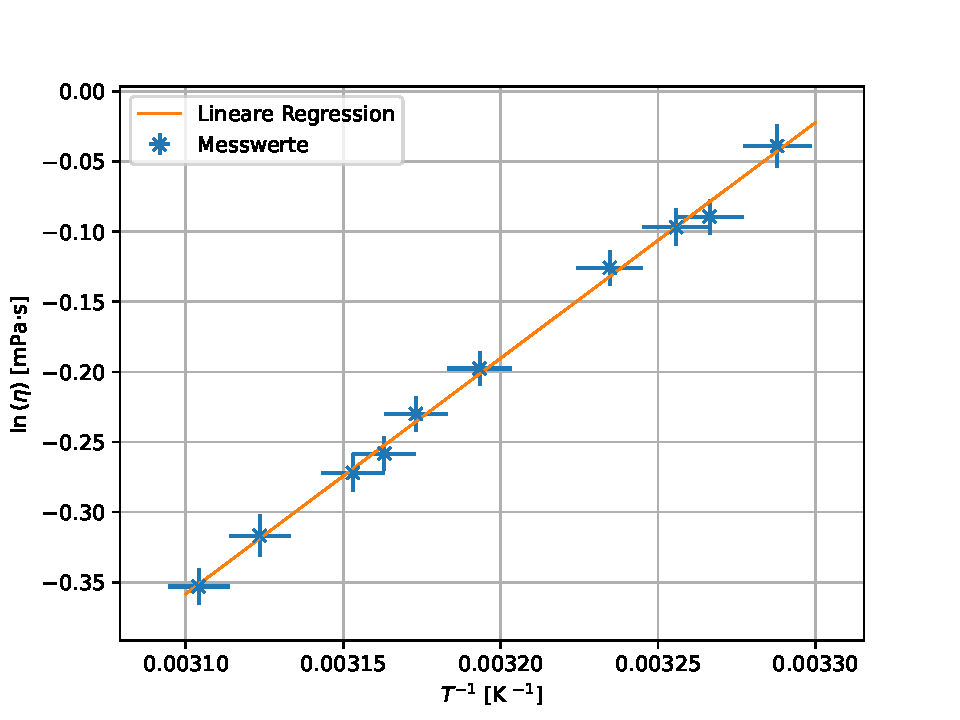
\includegraphics{plot.pdf}
  \caption{Plot.}
  \label{fig:plot}
\end{figure}

%Siehe \autoref{fig:plot}!